% pdflatex notes.tex 
\documentclass[twocolumn]{article}
\usepackage{amsfonts}
\usepackage{pifont}
\usepackage{hyperref}
\usepackage{tikz}
\usetikzlibrary{bayesnet}
\usepackage{amsmath}
\usepackage{amssymb}
\usepackage[most]{tcolorbox}
\usepackage{empheq}
\usepackage{geometry}
\geometry{a4paper, margin=1cm, includefoot}

\newtcbox{\mymath}[1][]{%
    nobeforeafter, math upper, tcbox raise base,
    enhanced, colframe=blue!30!black,
    colback=blue!15, boxrule=1pt,
    #1}

\begin{document}

\title{Notes on \href{https://www.youtube.com/watch?v=UwTQdOop-nU&list=PLwV-9DG53NDxU337smpTwm6sef4x-SCLv}{Visual Group Theory}}
\author{Rom Parnichkun}

\maketitle

\section{What is a group?}

A group is a set of actions satisfying some mild properties: deterministic, reversibility, and closure. The following lists the 4 axioms of groups.
\begin{itemize}
    \item There is a predefined list of \textit{actions} that never changes. \footnote{The list of actions required by this rule is our set of building blocks; called the generators.}
    \item Every action is reversible.
    \item Every action is deterministic.
    \item Any sequence of consecutive actions is also an action.
\end{itemize}

\section{Cayley graphs}

A Cayley graph is a mapping of a group; it is a visualization tool for Group theory.

\begin{figure}[h]
    \centering
    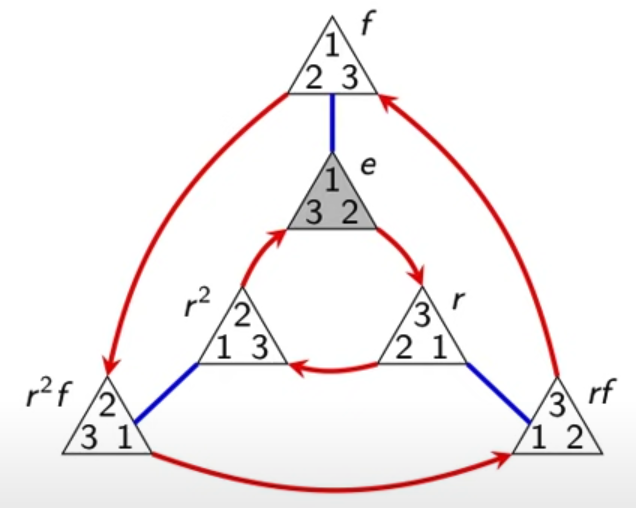
\includegraphics[width = 3in]{figure/cayley.png}
    \caption{An example cayley diagram.}
    \label{fig:cayley}
\end{figure}

\begin{figure}[h]
    \centering
    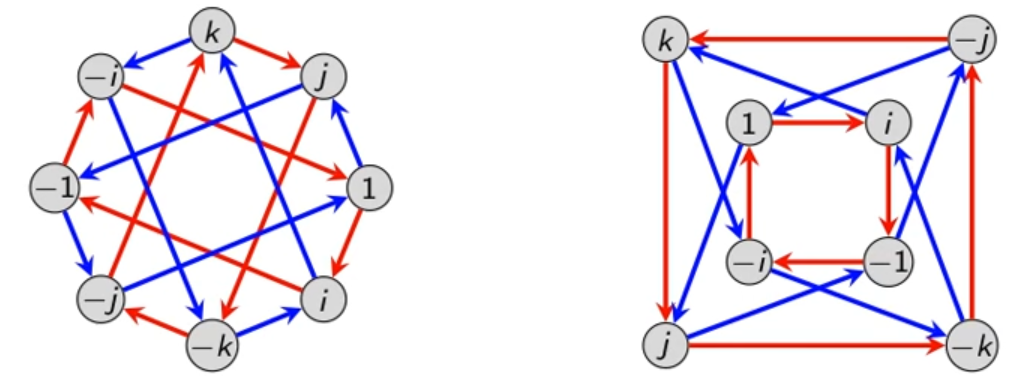
\includegraphics[width = 3in]{figure/cayley_quaternion.png}
    \caption{Quaternions can also be visualized with Cayley diagrams in two ways as $i^2 = j^2 = k^2 = -1$, and $ij = k, jk = i, ki = j, ji = -k, kj = -i, ik = -j$.}
    \label{fig:cayley}
\end{figure}

\textbf{Relations} in groups are formed when multiple paths can lead us to the same node.
In figure \ref{fig:cayley}, the relations are as follows:
\begin{equation}
    r^3 = e, r^{-1} = r^2, f^{-1} = f, rf = fr^2, r^2 f = fr.
\end{equation}

\textbf{Abelian} groups are groups in which the order of the actions is irrelaevant. The group is figure \ref{fig:cayley} is \textbf{non-abelian}.

\section{Groups of symmetries}

Intuitively, something is symmetrical when it looks the same from more than one point of view.

\begin{tcolorbox}[colback=blue!5!white,colframe=blue!15!white,coltitle=black, boxrule=0pt,title=Cayley's Theorem, drop shadow southeast, enhanced]
    Every group can be viewed as a collection of ways to rearrange some set of things.
\end{tcolorbox}

\subsection{How to make a group out of symmetries?}

Groups relate to symmetry because object's symmetries can be described using arrangements of the object's parts.

\begin{tcolorbox}[colback=blue!5!white,colframe=blue!15!white,coltitle=black, boxrule=0pt,title=Algorithm, drop shadow southeast, enhanced]
    \begin{enumerate}
        \item Identify all the parts of the object that are similar (e.g., the corners of an n-gon), and give each such part a different number.
        \item Consider the actions that may rearrange the numbered parts, but leave the object in the same physical space. (This collection of actions forms a group.)
    \end{enumerate}
\end{tcolorbox}

\section{Group presentation}

Groups can be presented in the following form:
\begin{equation}
    G = \langle \text{generators} \mid \text{relations}\rangle
\end{equation}
For example, the following is a presenation for $V_4$:
\begin{equation}
    V_4 = \langle a, b \mid a^2 = e, b^2 = e, ab = ba \rangle .
\end{equation}

\section{Multiplication tables}

If $g$ is a generator in a group $G$, then following the ``g-arrow" backwards is an actikon that we call its inverse, and denoted by $g^{-1}$.
\begin{equation}
    gg^{-1} = g^{-1}g = e,
\end{equation}
where $e$ is the identity action.

The following lists some of the inverses according to the example Cayley diagram in figure \ref{fig:cayley}.
\begin{itemize}
    \item $r^{-1} = r^2$
    \item $f^{-1} = f$
    \item $rf^{-1} = rf$
    \item $r^2f^{-1} = r^2f$
\end{itemize}

A \textbf{(group) multiplication table} shows how every pair of group actions combine.

\begin{figure}[h]
    \centering
    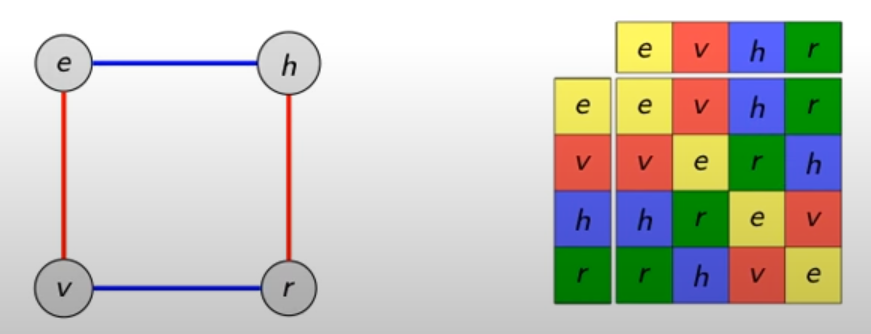
\includegraphics[width = 3in]{figure/multi_table.png}
    \caption{An example of a multiplication table.}
    \label{fig:multi}
\end{figure}

\begin{figure}[h]
    \centering
    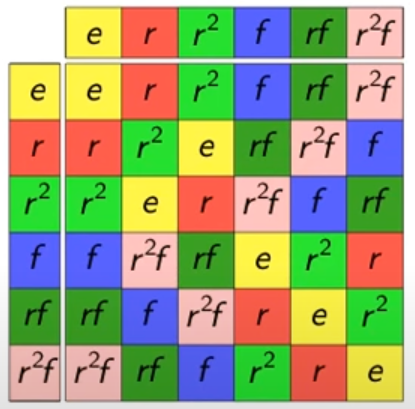
\includegraphics[width = 1.5in]{figure/multi_table2.png}
    \caption{An example of a multiplication table based on figure \ref{fig:cayley}. This group's representation is $D_3 = \langle r,f, \mid r^3 = e, f^2 = e, rf = fr^2 \rangle$.}
    \label{fig:multi2}
\end{figure}

\begin{tcolorbox}[colback=blue!5!white,colframe=blue!15!white,coltitle=black, boxrule=0pt,title=Notes on multiplication tables, drop shadow southeast, enhanced]
    \begin{itemize}
        \item The 1st column and 1st row repeat themselves. 
        \item Multiplication tables can reveal patterns that may be difficult to see otherwise.
        \item A group is abelian iff its multiplication table is symmetric about the ``main diagonal".
        \item In each row and each column, each group action occurs exactly once.
    \end{itemize}
\end{tcolorbox}

\section{The formal definition of a group}

We will call the mermbers of a group \textbf{elements}. In general, a group is a \textbf{set of elements} satisfying some set of properties.

\begin{tcolorbox}[colback=blue!5!white,colframe=blue!15!white,coltitle=black, boxrule=0pt,title=Definition of a binary operation, drop shadow southeast, enhanced]
    If $*$ is a \textbf{binary operation} on a set $S$, then $s * t \in S$ for all $s ,  t \in S$. In this case, we say that $s$ is \textbf{closed} under the operation $*$.
\end{tcolorbox}

\begin{itemize}
    \item Combining, or ``multiplying" two group elements is a binary operation. 
    \item Recall that Rule 4 says that any sequence of actions is an action. This ensures that the group is closed under the binary operation of multiplication.
    \item Multiplication tables are nice because they depict the group's binary operation in full.
    \item However, not every table with symbols in it is going to be the multiplication table for a group.
\end{itemize}

\begin{tcolorbox}[colback=blue!5!white,colframe=blue!15!white,coltitle=black, boxrule=0pt,title=Definition of a group, drop shadow southeast, enhanced]
    A set $G$ is a \textbf{group} if the following criteria are satisfied:
    \begin{itemize}
        \item There is a binary operation $*$ on $G$.
        \item $*$ is associative.
        \item There is an identity element $e \in G$. That is $e *g = g =  g*e$ for all $g \in G$.
        \item Every element $g \in G$ ahs an inverse, $g^{-1}$, satisfying $g*g^{-1} = e = g^{-1} * g$.
    \end{itemize}
\end{tcolorbox}

\begin{tcolorbox}[colback=blue!5!white,colframe=blue!15!white,coltitle=black, boxrule=0pt,title=Theorem, drop shadow southeast, enhanced]
    Every group has a \textit{unique} identity element.
\end{tcolorbox}

\section{Cyclic and Abelian groups}

\begin{tcolorbox}[colback=blue!5!white,colframe=blue!15!white,coltitle=black, boxrule=0pt,title=Definition, drop shadow southeast, enhanced]
    A group is \textbf{cyclic} if it can be generated by a single element. (think rotation)
\end{tcolorbox}

\begin{tcolorbox}[colback=blue!5!white,colframe=blue!15!white,coltitle=black, boxrule=0pt,title=Definition, drop shadow southeast, enhanced]
    The \textbf{order} of a group $G$ is the nubmer of distinct elements in $G$, denoted by $|G|$.
\end{tcolorbox}
For example, the cyclic group of order $n$ is denoted $C_n$ (or sometimes $Z_n$).

\subsection{Additive}

A common way to write elements in a cyclic group is with the integers $0,1,2,\dots,n-1$ where
\begin{itemize}
    \item 0 is the identity 
    \item 1 is the single counterclockwise fractional rotation ($\frac{2\pi}{n}$).
\end{itemize}

\subsection{Multiplicative}

Another natural choice of notation for cyclic groups. If $r$ is a generator then we can denote the n elements by 
\begin{equation}
    1,r, r^2,\dots,r^{n-1}
\end{equation}
Think of $r$ as a complex number $e^{2\pi i/n}$.
\begin{itemize}
    \item 1 is the identity
    \item r is the single counterclockwise fractional rotation.
\end{itemize}

\subsection{Orbits}

Every element in a group traces out an orbit. The orbit of figure \ref{fig:cayley} is shown in the table below.
\begin{table}[h]
    \centering
    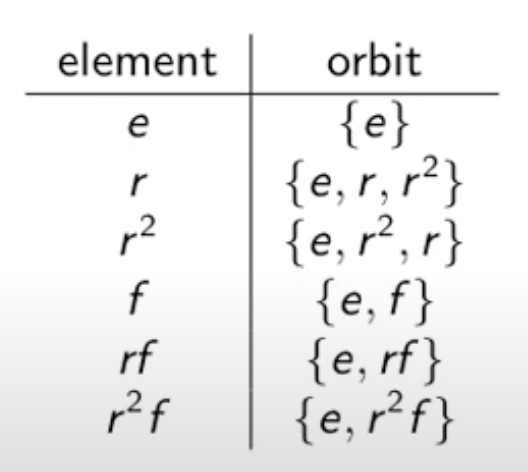
\includegraphics[width=2in]{figure/orbit.png}
\end{table}

\begin{tcolorbox}[colback=blue!5!white,colframe=blue!15!white,coltitle=black, boxrule=0pt,title=Definition, drop shadow southeast, enhanced]
    The \textbf{order} of an element $g \in G$, denoted $|g|$, is the size of its orbit. That is, $|g|:=|\langle g \rangle|$.
\end{tcolorbox}

\begin{tcolorbox}[colback=blue!5!white,colframe=blue!15!white,coltitle=black, boxrule=0pt,title=Remark, drop shadow southeast, enhanced]
    In any group $G$, the orbit of an element $g \in G$ is a \textbf{cyclic group} that ``sits inside" $G$. This is an example of a \textbf{subgroup}, which we will study in more detail later.
\end{tcolorbox}

\begin{tcolorbox}[colback=blue!5!white,colframe=blue!15!white,coltitle=black, boxrule=0pt,title=Definition, drop shadow southeast, enhanced]
    A group $G$ is \textbf{abelian} if $ab = ba$ for all $a,b \in G$.
\end{tcolorbox}
Abelian groups are someties referred to as \textbf{commutative}.

\section{Dihedral groups}

While cyclic groups describe 2D objects that only have rotational symmetry, \textbf{dihedral groups} describe 2D objects that have rotational and reflective symmetry. 

\begin{itemize}
    \item It is denoted as $D_n$.
    \item It has 2 generators, one for rotations, and another for reflections.
    \item An example presentation of $D_n$ is $D_n =langle r,f \mid r^n = e, f^2 = e, rfr = f \rangle$.
\end{itemize}
 
\section{Symmetric groups and Alternating groups}

\begin{tcolorbox}[colback=blue!5!white,colframe=blue!15!white,coltitle=black, boxrule=0pt,title=Definition, drop shadow southeast, enhanced]
    A \textbf{permulation} is an action that rearranges a collection of things.
\end{tcolorbox}

In order for the set of permutations of $n$ objects to form a group, we need to understand how to combine permutations.

\begin{tcolorbox}[colback=blue!5!white,colframe=blue!15!white,coltitle=black, boxrule=0pt,title=Definition, drop shadow southeast, enhanced]
    The group of all permutations of $n$ items is called the \textbf{symmetric group} and is denoted by $S_n$.
\end{tcolorbox}

\end{document}
